\section{Plan of Future Work}

Below is a high level plan for the work I have remaining. 

\subsection*{Implementation \& Testing}
In this phase I will use the agile development methodology to build my application. My sprints will all be structured into three phases:
\vspace{1mm}

\begin{enumerate}
  \item \textbf{Preparation} Deciding on the set of requirements to complete and making any initial design decisions and diagrams,
  \item \textbf{Implementation} Using test-driven development, I will work on requirements based on their prioritization, and
  \item \textbf{Review} I will discuss the completed work in that sprint including design choices, what was completed, and any issues.  
\end{enumerate}

\vspace{1mm}\noindent By using a preparation and review phase with each sprint, I can make detailed notes on my implementation as I go so when I come to write the full report I have a strong starting point.

\begin{figure}[ht]
  \centering
  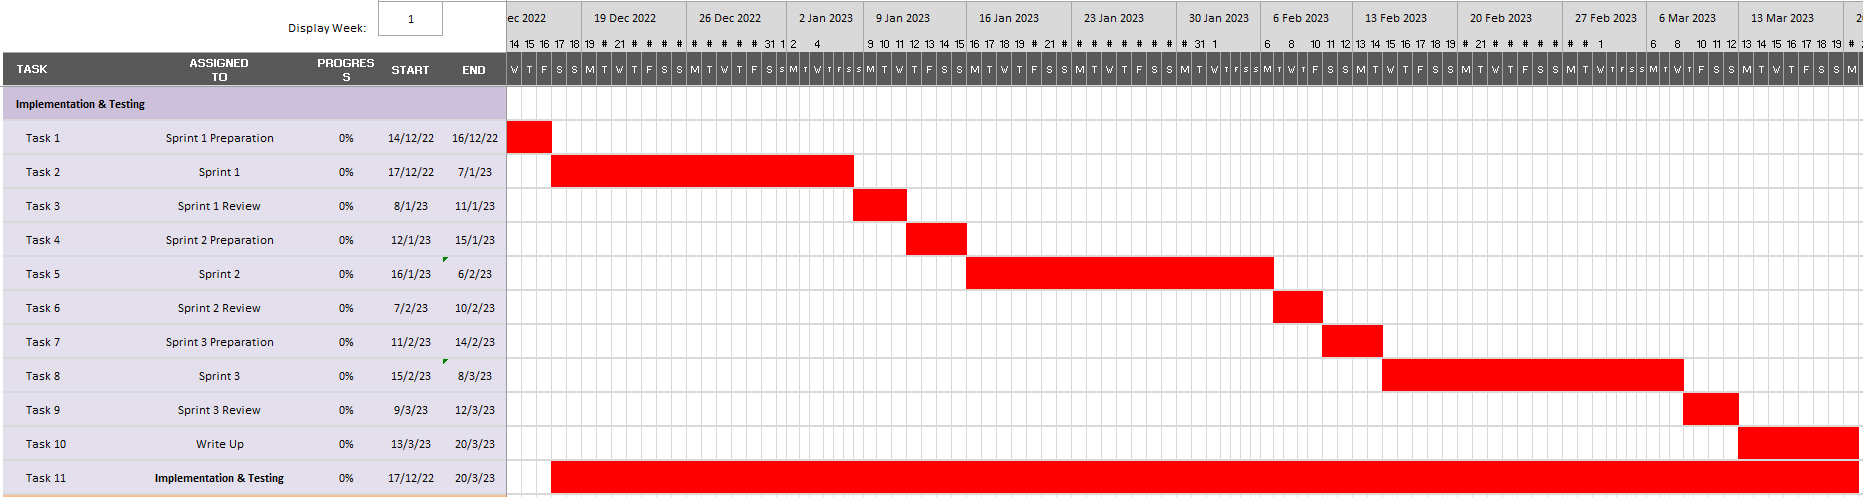
\includegraphics[width=\textwidth]{assets/images/charts/gantt/implementation-testing.png}
  \caption{The plan for my three sprints}
\end{figure}

\subsection*{Testing Strategy and Results}
This phase will consists of several sections:

\begin{enumerate}
  \item \textbf{Testing Strategy} The approach I used for writing tests throughout the implementation phase and how these were used to evaluate the completion of the requirements set out in Section~\ref{subsec:requirements}. 
  \item \textbf{Test Results} A report on the results of my automated and manual testing.
\end{enumerate}

\subsection*{Evaluation}
This phase will have me evaluating how successful my project was, as a whole, by focusing on several key areas:

\begin{enumerate}
  \item \textbf{Project Organisation} How successfully did I structure my time in this project?
  \item \textbf{Outcome of the Application} How successful was my application in regards to a solution to the problem set out in Section~\ref{sec:problem} and in terms of the requirements set out in Section~\ref{subsec:requirements}?
  \item \textbf{Limitations and Future Improvements} What were the limitations of my project and what would I change about it if I had more time or were to start again?
\end{enumerate}

\begin{figure}[ht]
  \centering
  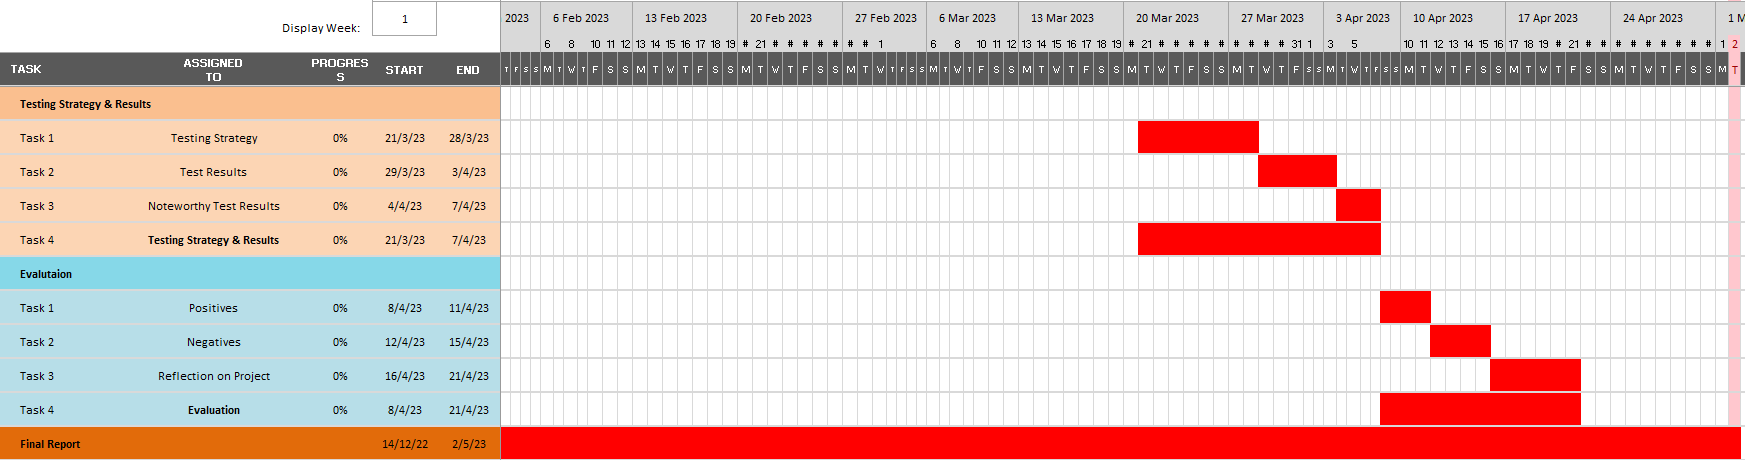
\includegraphics[width=\textwidth]{assets/images/charts/gantt/testing-evaluation.png}
  \caption{The plan for my testing and evaluation phases}
  \label{fig:final-gantt}
\end{figure}

\subsection*{Final Report}

I will be writing the first draft of my report throughout the project, aiming to finalise sections at the end of each phase of this project. Any leftover time at the end will be focused on finishing the report.
